\documentclass[border=10pt,varwidth]{standalone}
\usepackage{tikz}
\usetikzlibrary{shapes,arrows,shapes.multipart, positioning}

\begin{document}

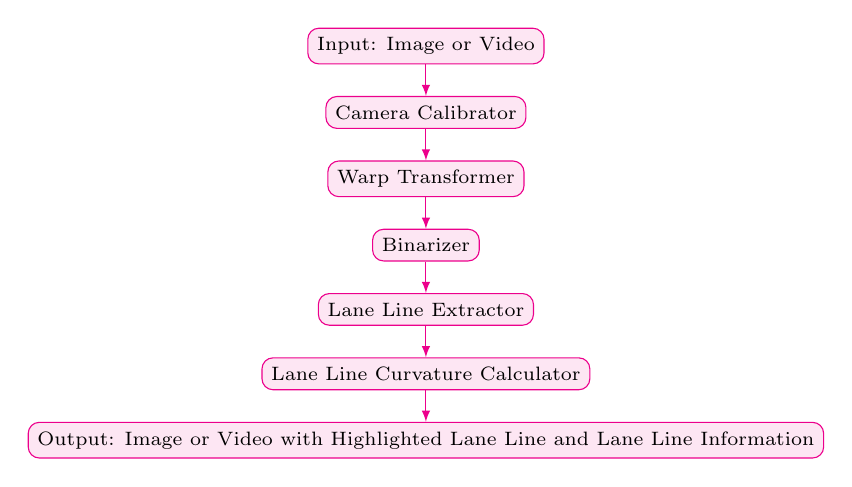
\begin{tikzpicture}
    \tikzset{
        node/.style = {rectangle, draw=magenta,  fill=magenta!10, thin, rounded corners},
        line/.style = {draw=magenta, thin, -latex},
        output/.style = {circle, draw=magenta,  fill=magenta!10, thin},
    }
    
    \node[node](input){\scriptsize Input: Image or Video};
    
    \node[node](camera)[below = 0.4cm of input]{\scriptsize Camera Calibrator};
    
    \node[node](shear)[below = 0.4cm of camera]{\scriptsize Warp Transformer};
    
    \node[node](crop)[below = 0.4cm of shear]{\scriptsize Binarizer};
    
    \node[node](flip)[below = 0.4cm of crop]{\scriptsize Lane Line Extractor};   
    
    \node[node](gamma)[below = 0.4cm of flip]{\scriptsize Lane Line Curvature Calculator}; 
    
    \node[node](resize)[below = 0.4cm of gamma]{\scriptsize Output: Image or Video with Highlighted Lane Line and Lane Line Information};
    
    \path [line] (input) -- (camera);
    \path [line] (camera) -- (shear);
    \path [line] (shear) -- (crop);
    \path [line] (crop) -- (flip);
    \path [line] (flip) -- (gamma);
    \path [line] (gamma) -- (resize);
    

\end{tikzpicture}

\end{document}
